\section{Subset attack} \label{subsec:subset-attack}
In the attempt to erase the fingerprint from the dataset, the attacker may release only a subset of tuples of a fingerprinted dataset. 
This is called a subset attack. 
In our attack model, we assume the attacker selects each tuple independently with probability \textit{p} to include it in the pirated dataset. 
We also assume no other updates on the dataset are applied and no other attacks performed. 

\subsection{AK Scheme}\label{subsubsec:subset-ak}
A subset attack succeeds when all embedded bits for at least one fingerprint bit are deleted. Assuming that each fingerprint bit $f_i$ is embedded $\omega_i$ times, then the probability that all embedded bits for $f_i$ are deleted is $(1-p)^{\omega_i}$. The probability that no valid fingerprint will be detected from the dataset is then 
\begin{equation} \label{eq:subset-attack-ak}
    fm = 1 - {\prod_{i=0}^{L-1}(1-(1-p)^{\omega_i})}.
\end{equation}

Table \ref{table:subset-attack-ak} shows the probability of a successful attack for different parameter $\gamma$ values. 
$p'=1-p$ denotes the probability that a single tuple is deleted, i.e. the approximate percentage of deleted tuples since the choice of deletion is made independently by the attacker. 
We set $\eta = 581,012$, $v=10$ (according to the properties of Forest Cover Type dataset that we use in empirical evaluation), $\xi=4$ and $L=96$.
We can see from the table that the subset attack only gets to the reasonable level of probability for success with more than at least 90\% deleted tuples, depending on $\gamma$. 
We have to take into account that as few as 1\% of the tuples in this example is around 5810 tuples, which for the attacker might still be the acceptable amount of tuples to release without authorisation and perform the successful subset attack if $\gamma$ is set high enough ($\gamma \geq 25$). 
In those cases where $p'$ is large, $\gamma$ should be set to the smaller value, since the probability for a successful subset attack decreases when $\gamma$ decreases for the same $p'$.
Therefore, we adapt $\gamma$ to prevent the subset attack.

\begin{table}[ht]
\centering
\caption{Probability of a successful subset attack on the AK Scheme}
\label{table:subset-attack-ak}
\begin{tabular}{|c|c|c|c|c|c|} 
 \hline
 & \textbf{$p'=70\%$} & \textbf{$p'=80\%$} & \textbf{$p'=90\%$} & \textbf{$p'=95\%$} & \textbf{$p'=99\%$}\\
 \hline
 $\gamma=6$ & 0 & 0 & 0 & 0 & 0.0038 \\
 \hline
 $\gamma=12$ & 0 & 0 & 0 & $5.6881 \times 10^{-10}$ & 0.4555 \\
 \hline
 $\gamma=25$ & 0 & 0 & $8.1088\times 10^{-10}$ & 0.0004 & 0.99985 \\
 \hline
 $\gamma=50$ & 0 & 0 & 0.0003 & 0.1761 & 1 \\
 \hline
  $\gamma=100$ & $4.877\times 10^{-8}$ & 0.0001 & 0.1586 & 0.9892 & 1 \\
 \hline
\end{tabular}
\end{table}


\paragraph{Experiments}
To present empirically the success of the subset attack, we performed the attack on the Forest dataset with $\eta = 581,012$ and $v=10$ using different parameter settings. 
The parameters are chosen the same way as shown in table \ref{table:subset-attack-ak} to be able to compare theoretical results with the empirical.
The experimental results are shown in table \Cref{table:subset-attack-ak-emp}.
Every experiment is run 500 times and parameters are set as presented in the table. 
We set $L=96$ and $\xi=4$ where the later does not affect the success of the subset attack.

We can see from the table \Cref{table:subset-attack-ak-emp} that the results roughly match our analysis. 
The best rate of success has the attacks where most of the tuples are deleted ($>$95\%) and the percentage of fingerprinted tuples is low ($\gamma$ is high). 
Therefore, we can argue that the AK Scheme is robust against subset attacks. 

\begin{table}[ht]
\centering
\caption{Experimental results of a subset attack success rate on the AK Scheme, using the Forest dataset}
\label{table:subset-attack-ak-emp}
\begin{tabular}{|c|c|c|c|c|c|} 
 \hline
 & \textbf{$p'=70\%$} & \textbf{$p'=80\%$} & \textbf{$p'=90\%$} & \textbf{$p'=95\%$} & \textbf{$p'=99\%$}\\
 \hline
 $\gamma=6$ & 0 & 0 & 0 & 0 & 0.004 \\
 \hline
 $\gamma=12$ & 0 & 0 & 0 & 0 & 0.5 \\
 \hline
 $\gamma=25$ & 0 & 0 & 0 & 0 & 1.0 \\
 \hline
 $\gamma=50$ & 0 & 0 & 0.002  & 0.194 &  1.0 \\
 \hline
  $\gamma=100$ & 0 & 0 & 0.20 & 0.9975 &  1.0 \\
 \hline
\end{tabular}
\end{table}


Note that our original dataset did not have a primary key. 
Instead, we added the attribute \textit{Id} to serve as the primary key. 
For simplicity purposes, the $Id$ values in the experiments are represented by the sequence number of the tuple.
Furthermore, although during subset attack the attacker removes some tuples, we assume that the primary key of every preserved tuple will not change.
In case the primary key is removed or manipulated, the recreation of one is crucial for the defence against the subset attack.
Availability of the original dataset simplifies the process of recreating the primary key. 
A simple matching algorithm can be applied to the suspect dataset that compares values of bit positions which are not being selected for marking in the fingerprinting process to the same set of bit positions in the original data. 
This approach might be flawed by having multiple primary key value candidates for a single tuple. 
In that case, the additional decision step based on the similarity of the bits used for marking can be applied.
Alternatively, the virtual primary key construction technique proposed in \cite{li2003constructing} can be used to generate the primary keys and does not require the presence of the original dataset. 
Primary keys are generated from the unmarked parts or data and the owner's secret key using a cryptographic hash function. Without knowing the secret key, recreating the primary key values is unfeasible. 

\subsection{Block Scheme}
For the Block Scheme detection algorithm, it is crucial to have the same number of tuples and attributes and their correct order in the suspicious database. Otherwise, we cannot detect a valid fingerprint. 
When the attacker removes the chosen tuples, the defence has to replace the deleted one with the corresponding ones from the original dataset. 
In our analysis we formulate the deletion of each tuple as an independent trial with two possible outcomes whose probabilities remain the same through the trials (\textit{Bernoulli trial}). Furthermore, with $B(k;n.p)$ we denote the probability of having at least $k$ successes in $n$ trials with probability $p$ of success.  
The detection algorithm will be able to detect the correct fingerprint if every fingerprint bit $f_i$ occurs at least $\lfloor\tau\omega_i\rfloor$ times in the suspicious dataset.
It means that at least $\lfloor(1-\tau)\omega_i\rfloor$ embedded bits for some fingerprint bit have to be deleted for the attack to succeed.  
If the attacker examines each tuple independently and selects it for inclusion in the pirated database (i.e. deletes it with probability $p'=1-p$), the probability that the fingerprint bit $f_i$ cannot be detected is $B(\lfloor(1-\tau)\omega_i\rfloor;\omega_i,p')$.
Note that each fingerprint bit in the Block Scheme is embedded either $\omega$ or $\omega-1$ times, so we approximate this value to $\omega$ for the convenience.
Then the probability that the detection algorithm will fail to extract the fingerprint is 
\begin{equation}
    fm=1-(1-B(\lfloor(1-\tau)\omega_i\rfloor;\omega_i,p'))^L
\end{equation}

Table \ref{table:subset-attack-block} shows the probabilities of successful subset attack under different values of parameter $\beta$ and different probabilities $p'$. For calculations we use dataset of size $\eta = 581,012$ and $v=10$ attributes, for purpose of comparing these results with experimental results.
The other parameters are set as follows: $\xi=3$, $L=96$ and $\tau=0.5$.

\begin{table}[ht]
\centering
\caption{Probability of a successful subset attack on the Block Scheme}
\label{table:subset-attack-block}
\begin{tabular}{|c|c|c|c|c|} 
 \hline
 & \textbf{$p'=30\%$} & \textbf{$p'=40\%$} & \textbf{$p'=45\%$} & \textbf{$p'=50\%$}\\
 \hline
 $\beta=5$ & 0 & 0 & 0 & 1.0 \\
 \hline
 $\beta=10$ & 0 & 0 & 0.001 & 1.0 \\
 \hline
 $\beta=15$ & 0 & $6.8233\times10^{-7}$ & 0.2320 & 1.0 \\
 \hline
 $\beta=20$ & 0 & $9.7949\times10^{-4}$ & 0.8301 & 1.0\\
 \hline
  $\beta=30$ & $2.0832\times10^{-7}$ & 0.2151 & 0.9998 & 1.0 \\
 \hline
\end{tabular}
\end{table}

\paragraph{Experiments}
We present the empirical results of the success of a subset attack on the Block Scheme. 
The experiments are run on Forest dataset of size $\eta = 581,012$ and $v=10$ attributes, with parameters $\xi=3$, $L=96$ and $\tau=0.5$.
We measure success of the attack for $p'=\{0.30, 0.40, 0.45, 0.50\}$ and $\beta=\{5,10,15,20,30\}$.
We run each experiment 500 times and summarise the number of successes/fails of the attack.
In table \ref{table:subset-attack-block-emp} the empirical results are presented.

\begin{table}[ht]
\caption{Probability of a successful subset attack on the Block Scheme}
\label{table:subset-attack-block-emp}
\centering
\begin{tabular}{|c|c|c|c|c|} 
 \hline
 & \textbf{$p'=30\%$} & \textbf{$p'=40\%$} & \textbf{$p'=45\%$} & \textbf{$p'=50\%$}\\
 \hline
 $\beta=5$ & 0 & 0 & 0 & 1.0 \\
 \hline
 $\beta=10$ & 0 & 0 & 0.008 & 1.0 \\
 \hline
 $\beta=15$ & 0 & 0 & 0.356 & 1.0 \\
 \hline
 $\beta=20$ & 0 & 0.002 & 0.914 & 1.0\\
 \hline
  $\beta=30$ & 0 & 0.196 & 1.0 & 1.0 \\
 \hline
\end{tabular}
\end{table}

For $\beta$ values 5, 10 and 15, up to 40\% of the arbitrary tuples can be deleted and it will not affect the detection of the fingerprint. 
Larger values of $\beta$ tolerate around 30\% of the deleted tuples. 
Compared to the theoretical results in \Cref{table:subset-attack-block}, the experimental results are very similar.

\subsection{Two-level Fingerprinting Scheme}
The Two-level Fingerprinting scheme provides two levels of marking patterns; the first one that can verify the owner and the second one verifying the recipient of the dataset.
When the attacker removes a subset of tuples and releases the remainder, the fingerprint is affected in two ways:
\begin{enumerate}
    \item It might be impossible to trace back the owner but the owner can claim the ownership
    \item It might be impossible both to trace back the owner and to claim the ownership
\end{enumerate}

\paragraph{Experiments}

\begin{figure}
\centering
    \subfloat[$\gamma_1=100$]{{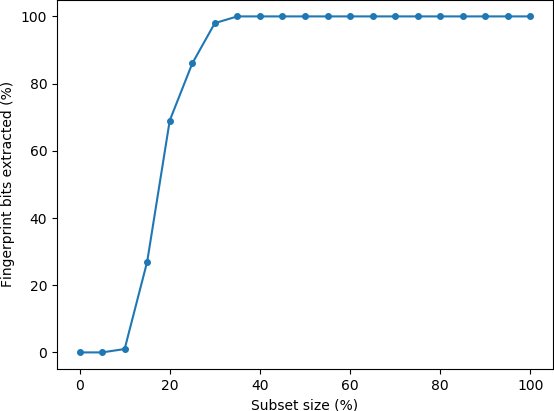
\includegraphics[width=6.7cm]{Figures/subset_attack_two-level_gamma100.png} }}
    \qquad
    \subfloat[$\gamma_1=50$]{{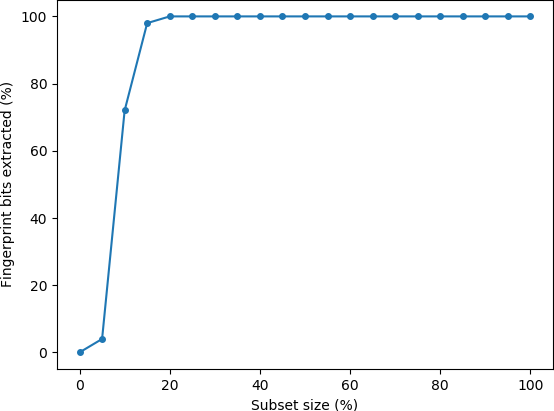
\includegraphics[width=6.7cm]{Figures/subset_attack_two-level_gamma50.png} }}
    \caption{Fingerprint extraction in a subset attack}
    \label{fig:subset-attack-two-level-fp-bits}
\end{figure}

The attack may cause that the extraction process does not manage to extract all the fingerprint bits correctly.
We can see from \Cref{fig:subset-attack-two-level-fp-bits}(a) that even if only around 35\% of the tuples are released by the malicious buyer, all fingerprint bits are still correctly extracted. 
The robustness of this scheme can be improved by changing the value of $\gamma_1$. 
\Cref{fig:subset-attack-two-level-fp-bits}(b) shows the results for a smaller $\gamma_1$, i.e. for the increased number of marks in the data that can be used to verify the ownership. 
For this parameter setting, the scheme is more robust against the subset attack, and even from only 20\% of the data, all the correct fingerprint bits can be extracted. 
For this experiments, we used the fingerprint of length $L=96$ and the bit significance level of each bit $\alpha_2$ is 0.01 (the confidence level is 99\%).

\begin{table}[ht]
    \centering
    \caption{Success of the subset attack on Two-level Fingerprinting Scheme}
    \label{tab:subset-attack-two-level}
    \begin{tabular}{|c|c|c|c|c|c|c|}
        \hline
         & $p'=60\%$ & $p'=70\%$ & $p'=80\%$ & $p'=90\%$ & $p'=95\%$ & $p'=99\%$ \\
         \hline
         $\gamma_1 = \gamma_2 = 10$ & 0 & 0 & 0 & 0 & 0 & 1.0 \\
         \hline
         $\gamma_1 = \gamma_2 = 25$ & 0 & 0 & 0 & 0.04 & 1.0 & 1.0 \\
         \hline
         $\gamma_1 = \gamma_2 = 50$ & 0 & 0 & 0.04 & 0.98 & 1.0 & 1.0 \\
         \hline
         $\gamma_1 = \gamma_2 = 100$ & 0 & 0.74 & 1.0 & 1.0 & 1.0 & 1.0 \\
         \hline
         $\gamma_1 = \gamma_2 = 200$ & 1.0 & 1.0 & 1.0 & 1.0 & 1.0 & 1.0 \\
         \hline
    \end{tabular}
\end{table}

Let us consider the setting where $\gamma_1=50$ and $\gamma_2=50$. For $p<20\%$ ($p'>80\%$; the attacker removes more than 80\% of the tuples) some bit positions will be unknown. For $p=15\%$ on average 2 out of 96 bit positions cannot be detected, creating $2^2$ fingerprint candidates. 
The fingerprint verification process may still select the correct fingerprint out of $2^2$ possible ones and the extraction algorithm finds the malicious buyer successfully. 
In the same setting, when 90\% of the tuples are removed, the algorithm correctly extracts 72\% correct fingerprint bits, or 69 out of 96. 
This is not enough for the fingerprint verification algorithm to verify any fingerprint and the detection algorithm fails. 
See the \Cref{tab:subset-attack-two-level} where the success of the subset attack is recorded. 
The experiments are run using Forest Cover Type data. 
The results in the table confirm that although not all fingerprint bits are extracted, the attack is not 100\% successful. 

\begin{figure}
    \centering
    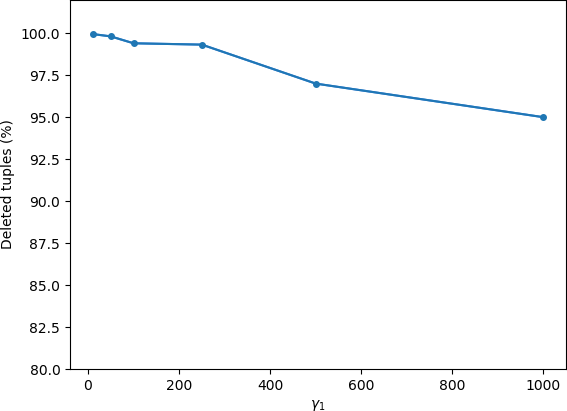
\includegraphics[width=0.7\textwidth]{Figures/subset_attack_two-level-ownership-ver.png}
    \caption{Ownership verification in a subset attack}
    \label{fig:subset-attack-ownership-verification}
\end{figure}

The first level of the embedding process provides the ownership verification even for cases when the correct fingerprint cannot be extracted. 
So, although the owner cannot trace the source of unauthorised leakage of data, she can claim the ownership. The mark created in this process is very robust. See in the \Cref{fig:subset-attack-ownership-verification} that even from the very small percentage of the data (<5\%), the detection algorithm will verify the owner with confidence level 99\% ($\alpha_1=0.01$).
The experiments are run even for the very big values of $\gamma_1$. 
For the settings where our experiments show high probabilities of extracting the right fingerprint from the small chunks of data, i.e $10<\gamma_1,\gamma_2<100$, up to 99\% of the tuples can be deleted and ownership can still be claimed.      

\subsection{Fingerprinting scheme for categorical data}
The fingerprinting scheme for categorical data complements the AK Scheme and for subset attack, we can refer to \Cref{eq:subset-attack-ak} as a starting point for analysis. 
The important difference between AK Scheme and scheme for categorical data is the introduction of modulo operation as one of the steps. 
We mentioned before in \Cref{subsec:fingerprinting-scheme-categorical} that we trade the strength of detection algorithm for fingerprinting categorical data successfully. 
This means that additional modulo operation step in the fingerprint insertion phase causes errors in the detection phase that cannot be avoided. 
Having errors in unaffected fingerprinting scheme increases the vulnerability of the scheme to attacks. 
Therefore, the \Cref{eq:subset-attack-ak} lacks influence of modulo operation in order to be credible. 
\Cref{tab:subset-attack-adult} shows the theoretical success of the subset attack on the dataset with $\eta = 30,162$ rows (convenient for comparison to experimental results on Adult dataset) if the effects of modulo are not taken into account, using \Cref{eq:subset-attack-ak}.
$\omega_i$ is approximated to $\eta/(\gamma*L)$ and $L=80$. 
Value 0 represents the perfect resistance to the subset attack, and 1 is the perfect success of the subset attack, i.e. the scheme completely failing to defend against it.

\begin{table}[ht]
    \centering
    \caption{Theoretical success rate of a subset attack on the fingerprinting scheme for categorical data, using the Adult data}
    \label{tab:subset-attack-adult}
    \begin{tabular}{|c|c|c|c|c|c|c|}
         \hline
        & \textbf{$p'=30\%$} & \textbf{$p'=60\%$} & \textbf{$p'=80\%$} & \textbf{$p'=90\%$} & \textbf{$p'=95\%$} & \textbf{$p'=99\%$}\\
        \hline
        $\gamma=3$ & 0.0 & 0.0 & 0.0 & 0.0001 & 0.1174 & 1.0 \\
        \hline
        $\gamma=6$ & 0.0 & 0.0 & 0.0001 & 0.0996 & 0.9601 & 1.0 \\
        \hline
        $\gamma=12$ & 0.0 & 0.0 & 0.0762 & 0.9555 & 1.0 & 1.0 \\
        \hline
        $\gamma=25$ & $1.15\times10^{-6}$ & 0.3166 & 0.9430 & 1.0 & 1.0 & 1.0 \\
        \hline
        $\gamma=50$ & 0.0052 & 0.7421 & 1.0 & 1.0 & 1.0 & 1.0 \\
         \hline
        $\gamma=100$ & 0.4783 & 0.9999 & 1.0 & 1.0 & 1.0 & 1.0 \\
         \hline
     \end{tabular}
\end{table}

\paragraph{Experiments}
The experiments are made on the Adult dataset as it is the dataset containing categorical attributes. 
We measure the success of subset attack over 500 runs and parameters set as follows: $L=80$, $\xi=1$, $\tau=0.5$, $\gamma=\{3,6,12,25,50,100\}$ and $p'=\{0.30,0.60,0.80,0.90,0.95,0.99\}$, where $p'$ represents the percentage of tuples that are deleted.


\begin{table}[ht]
    \centering
    \caption{Experimental results of the subset attack success rate on the fingerprinting scheme for categorical data, using the Adult data}
    \label{tab:subset-attack-adult-experimental}
    \begin{tabular}{|c|c|c|c|c|c|c|}
         \hline
        & \textbf{$p'=30\%$} & \textbf{$p'=60\%$} & \textbf{$p'=80\%$} & \textbf{$p'=90\%$} & \textbf{$p'=95\%$} & \textbf{$p'=99\%$}\\
        \hline
        $\gamma=3$ & 0.0 & 0.0 & 0.0 & 0.004 & 0.22 & 1.0 \\
        \hline
        $\gamma=6$ & 0.08 & 0.18 & 0.20 & 0.354 & 0.954 & 1.0\\
        \hline
        $\gamma=12$ & 0.078 & 0.0 & 0.212 & 0.97 & 1.0 & 1.0 \\
        \hline
        $\gamma=25$ & 0.012 & 0.284 & 0.99 & 1.0 & 1.0 & 1.0 \\
        \hline
        $\gamma=50$ & 0.346 & 1.0 & 1.0 & 1.0 & 1.0 & 1.0 \\
         \hline
        $\gamma=100$ & 0.976 & 1.0 & 1.0 & 1.0 & 1.0 & 1.0 \\
         \hline
     \end{tabular}
\end{table}

\Cref{tab:subset-attack-adult} and \Cref{tab:subset-attack-adult-experimental} share the same parameter settings for calculating the success of a subset attack on the Adult dataset, however, in latter the rate of success is larger overall.
Although the detection algorithm can detect the correct fingerprint from the full set of tuples, the errors introduced by modulo operation are enhancing the success of the attack. 
Therefore, only for small values of $\gamma$, the scheme is resistant to subset attack if the large portion of tuples is not deleted. 


